% Template for PLoS
% Version 3.5 March 2018
%
% % % % % % % % % % % % % % % % % % % % % %
%
% -- IMPORTANT NOTE
%
% This template contains comments intended
% to minimize problems and delays during our production
% process. Please follow the template instructions
% whenever possible.
%
% % % % % % % % % % % % % % % % % % % % % % %
%
% Once your paper is accepted for publication,
% PLEASE REMOVE ALL TRACKED CHANGES in this file
% and leave only the final text of your manuscript.
% PLOS recommends the use of latexdiff to track changes during review, as this will help to maintain a clean tex file.
% Visit https://www.ctan.org/pkg/latexdiff?lang=en for info or contact us at latex@plos.org.
%
%
% There are no restrictions on package use within the LaTeX files except that
% no packages listed in the template may be deleted.
%
% Please do not include colors or graphics in the text.
%
% The manuscript LaTeX source should be contained within a single file (do not use \input, \externaldocument, or similar commands).
%
% % % % % % % % % % % % % % % % % % % % % % %
%
% -- FIGURES AND TABLES
%
% Please include tables/figure captions directly after the paragraph where they are first cited in the text.
%
% DO NOT INCLUDE GRAPHICS IN YOUR MANUSCRIPT
% - Figures should be uploaded separately from your manuscript file.
% - Figures generated using LaTeX should be extracted and removed from the PDF before submission.
% - Figures containing multiple panels/subfigures must be combined into one image file before submission.
% For figure citations, please use "Fig" instead of "Figure".
% See http://journals.plos.org/plosone/s/figures for PLOS figure guidelines.
%
% Tables should be cell-based and may not contain:
% - spacing/line breaks within cells to alter layout or alignment
% - do not nest tabular environments (no tabular environments within tabular environments)
% - no graphics or colored text (cell background color/shading OK)
% See http://journals.plos.org/plosone/s/tables for table guidelines.
%
% For tables that exceed the width of the text column, use the adjustwidth environment as illustrated in the example table in text below.
%
% % % % % % % % % % % % % % % % % % % % % % % %
%
% -- EQUATIONS, MATH SYMBOLS, SUBSCRIPTS, AND SUPERSCRIPTS
%
% IMPORTANT
% Below are a few tips to help format your equations and other special characters according to our specifications. For more tips to help reduce the possibility of formatting errors during conversion, please see our LaTeX guidelines at http://journals.plos.org/plosone/s/latex
%
% For inline equations, please be sure to include all portions of an equation in the math environment.
%
% Do not include text that is not math in the math environment.
%
% Please add line breaks to long display equations when possible in order to fit size of the column.
%
% For inline equations, please do not include punctuation (commas, etc) within the math environment unless this is part of the equation.
%
% When adding superscript or subscripts outside of brackets/braces, please group using {}.
%
% Do not use \cal for caligraphic font.  Instead, use \mathcal{}
%
% % % % % % % % % % % % % % % % % % % % % % % %
%
% Please contact latex@plos.org with any questions.
%
% % % % % % % % % % % % % % % % % % % % % % % %

\documentclass[10pt,letterpaper]{article}
\usepackage[top=0.85in,left=2.75in,footskip=0.75in]{geometry}

% amsmath and amssymb packages, useful for mathematical formulas and symbols
\usepackage{amsmath,amssymb}

% Use adjustwidth environment to exceed column width (see example table in text)
\usepackage{changepage}

% Use Unicode characters when possible
\usepackage[utf8x]{inputenc}

% textcomp package and marvosym package for additional characters
\usepackage{textcomp,marvosym}

% cite package, to clean up citations in the main text. Do not remove.
% \usepackage{cite}

% Use nameref to cite supporting information files (see Supporting Information section for more info)
\usepackage{nameref,hyperref}

% line numbers
\usepackage[right]{lineno}

% ligatures disabled
\usepackage{microtype}
\DisableLigatures[f]{encoding = *, family = * }

% color can be used to apply background shading to table cells only
\usepackage[table]{xcolor}

% array package and thick rules for tables
\usepackage{array}

% create "+" rule type for thick vertical lines
\newcolumntype{+}{!{\vrule width 2pt}}

% create \thickcline for thick horizontal lines of variable length
\newlength\savedwidth
\newcommand\thickcline[1]{%
  \noalign{\global\savedwidth\arrayrulewidth\global\arrayrulewidth 2pt}%
  \cline{#1}%
  \noalign{\vskip\arrayrulewidth}%
  \noalign{\global\arrayrulewidth\savedwidth}%
}

% \thickhline command for thick horizontal lines that span the table
\newcommand\thickhline{\noalign{\global\savedwidth\arrayrulewidth\global\arrayrulewidth 2pt}%
\hline
\noalign{\global\arrayrulewidth\savedwidth}}


% Remove comment for double spacing
%\usepackage{setspace}
%\doublespacing

% Text layout
\raggedright
\setlength{\parindent}{0.5cm}
\textwidth 5.25in
\textheight 8.75in

% Bold the 'Figure #' in the caption and separate it from the title/caption with a period
% Captions will be left justified
\usepackage[aboveskip=1pt,labelfont=bf,labelsep=period,justification=raggedright,singlelinecheck=off]{caption}
\renewcommand{\figurename}{Fig}

% Use the PLoS provided BiBTeX style
% \bibliographystyle{plos2015}

% Remove brackets from numbering in List of References
\makeatletter
\renewcommand{\@biblabel}[1]{\quad#1.}
\makeatother



% Header and Footer with logo
\usepackage{lastpage,fancyhdr,graphicx}
\usepackage{epstopdf}
%\pagestyle{myheadings}
\pagestyle{fancy}
\fancyhf{}
%\setlength{\headheight}{27.023pt}
%\lhead{
\includegraphics[width=2.0in]{PLOS-submission.eps}}
\rfoot{\thepage/\pageref{LastPage}}
\renewcommand{\headrulewidth}{0pt}
\renewcommand{\footrule}{\hrule height 2pt \vspace{2mm}}
\fancyheadoffset[L]{2.25in}
\fancyfootoffset[L]{2.25in}
\lfoot{\today}

%% Include all macros below

\newcommand{\lorem}{{\bf LOREM}}
\newcommand{\ipsum}{{\bf IPSUM}}


\usepackage{booktabs}
\usepackage{longtable}
\usepackage{array}
\usepackage{multirow}
\usepackage{wrapfig}
\usepackage{float}
\usepackage{colortbl}
\usepackage{pdflscape}
\usepackage{tabu}
\usepackage{threeparttable}
\usepackage{threeparttablex}
\usepackage[normalem]{ulem}
\usepackage{makecell}
\usepackage{xcolor}



\usepackage{forarray}
\usepackage{xstring}
\newcommand{\getIndex}[2]{
  \ForEach{,}{\IfEq{#1}{\thislevelitem}{\number\thislevelcount\ExitForEach}{}}{#2}
}

\setcounter{secnumdepth}{0}

\newcommand{\getAff}[1]{
  \getIndex{#1}{UC Davis,UNH}
}

\providecommand{\tightlist}{%
  \setlength{\itemsep}{0pt}\setlength{\parskip}{0pt}}

\begin{document}
\vspace*{0.2in}

% Title must be 250 characters or less.
\begin{flushleft}
{\Large
\textbf\newline{Peaks and valleys of prolatin-related gene expression during pigeon
parental care stages} % Please use "sentence case" for title and headings (capitalize only the first word in a title (or heading), the first word in a subtitle (or subheading), and any proper nouns).
}
\newline
% Insert author names, affiliations and corresponding author email (do not include titles, positions, or degrees).
\\
Rayna M Harris\textsuperscript{\getAff{UC Davis}}\textsuperscript{*},
Suzanne Austin\textsuperscript{\getAff{UC Davis}},
Andrew Lang\textsuperscript{\getAff{UNH}},
Matthew MacManes\textsuperscript{\getAff{UNH}},
Rebecca M Calisi\textsuperscript{\getAff{UC Davis}}\\
\bigskip
\textbf{\getAff{UC Davis}}UC Davis, Davis, CA\\
\textbf{\getAff{UNH}}UNH, smalltown, NH\\
\bigskip
* Corresponding author: rmharris@ucdavis\\
\end{flushleft}
% Please keep the abstract below 300 words
\section*{Abstract}
The goal of this research was to provide the most comprehensive gene
expression profile of gene expression activity in the HPG axis of male
and female rock doves to provide a deeper undertand of how the
reproductive axis response to typical behavioral transitions associated
with parental care. Here we used RNA sequencing to measure gene activity
at 8 stages of the parental care cyle from nest building, to egg
incubation, and through nestling care. Non-parental groups were added as
controls, but gene expressions differences were assesed between and
across all time points. The three tissue have unique signatures, but
within each tissue we find minial sex differences. The pitutary samples
displacy the msot plasticity in gene expression, with many changes in
gene expression mirroring the typical rise and fall of circulating
prolatin that peaks when chicks hatch. Our analysis provides new insight
into how suites of genes respond in concert to the demands of offspring
care. This data can be used to develop and test hypotheses about the
mechanism regulating parental care behavior.

% Please keep the Author Summary between 150 and 200 words
% Use first person. PLOS ONE authors please skip this step.
% Author Summary not valid for PLOS ONE submissions.

\linenumbers

% Use "Eq" instead of "Equation" for equation citations.
\hypertarget{introduction}{%
\section{Introduction}\label{introduction}}

Understanding the mechanisms underlying parental care are critical to
circumventing issues with parent-newborn bonding as well, where ultimate
explanations are obvious, but specific mechanisms remain elusive. The
rock dove (\emph{Columba livia}) is an ideal system to characterize
changes in genetic expression during parental care transitions because:
1) ample genomic resources are available (Gillespie et al.~2013),
including a complete annotated genome assembly {[}1{]} and methodology
concerning reproductive physiology and behavior (Dong et al.~2012); and
2) rock doves are prolific, year-round breeders that thrive in
captivity, making observation, manipulation, and sampling highly
feasible year-round. Rock doves are socially monogamous and offer
bi-parental care, making inter- and intra-sexual comparisons possible.
Birds offer two important behavioral transition points into parental
care: the incubation of eggs and the caring for chicks. This produces
two unique opportunities to study how the brain transitions into two
different suites of parental care behaviors. Additionally, rock doves
exhibit a parental care strategy analogous to mammals in that they, too,
`lactate' to feed their young (Gillespie et al.~2011, 2012). This
lactation, unlike simple regurgitation of food, consists of the
production and sloughing off of skin cells inside the crop sac of
females and males, creating a protein-rich milk-like substance on which
they rear their chicks. Many functional similarities between rock dove
and mammalian lactation exist concerning the mediation of this event by
the hormone prolactin (Dumont 1965). Additionally, like mammalian milk,
rock dove milk delivers essential immunoglobulins and nutritional
benefits to young, aiding in their immune function and development of
microbiota {[}2{]}. Thus, because rock doves incubate eggs and exhibit
mammalian-like mediation and function of lactation for young, they have
the potential to serve as a powerful theoretical bridge to understand
the neurobiology of both avian and mammalian transitions into parental
care. Our working hypothesis is that distinct changes in transcription
occur in the brain at the anticipation of, during, and in response to
two different types of parental care: incubation behavior and hatchling
care.

\hypertarget{materials-and-methods}{%
\section{Materials and Methods}\label{materials-and-methods}}

Sexually mature male and female rock doves were housed together in
rooftop aviaries on the Barnard Campus. Natural male-female pairings
permitted, and small observation windows behind each nest box (64 boxes
total) facilitate observations nest building, egg laying, chick
hatching, and nesting care every morning from 0900-1100 (correct time?).
On specific collection days (Fig 1A, needs to be updated), truck blook,
the hypothalamus, the pituitary, and the gonads were collected following
common protocols used to sample tissue from birds (Fig 1B). Tissue
collection, RNA isolation, cDNA library preparation, sequencing, quality
control, and read processing were done as described in Calisi et
al.~2018, Lang et al 2019, and Austin et al 2019.

We used EdgeR determine the greatest contributor to variance in gene
expression in the full dataset. Then, we used EdgeR and DESeq2 were used
to calculate statistical differnces in gene expression between each
transition within a given tissue. All subsequent analyses were
conducting using variance stabilized data from the DESeq2 model. A
linear discriminant analysis was used to determine the confidence with
which we could predict the parental care stage of a sample based on it's
global gene expression profile. WGCNA was used to identify genes who's
expression was correlated with specific candidate genes of interest.

\hypertarget{results}{%
\section{Results}\label{results}}

We found that the majority of the variation in the full dataset could be
attributed to tissue, with only a notable sex differnce existing between
the female ovaries and the male testies (Fig. 2).

Thousands of genes were found to be differentially expressed between the
non-parental control group and the nest-building group (Table 1, Fig.
3). Within the time course of parental care, fewer than 1000 genes
change there expression over the course of a few days, with the most
pronounced difference in toltal number of changes occuring in the female
pituitary between incubation days 9 and 17 (Table 1, Fig. 3).

Even though we have a large sample size of roughly 12 samples per tissue
per sex, the differences between all 8 sampled parental time points are
so small, that we are only able to predict the stage using gene
expression along 40\%, 30\% and 27\% of the time in the pituiary, gonads
and hypothalamus, respectively (Fig 4A). However, if we group the
parental stages into anticipatory (control, nest building), egg care
(lay and incubation days), and nestling care (hatch and nesting days),
we incrase our ability to detect parental stage to 47\%, 43\%, and 37
pituiary, hypothalamus and gonads, respectively (Fig 4B).

Gene expression of prlactin (\emph{PRL})in the pitutiary, but not the
hypothalamus follows the characteristic dip in expression relative to
non-parental controls during early incubation then spikes the day before
hatch and peaks at hatch (Fig 5).

Hundreds of genes follow this same, prolactin-associated pattern of
expression in the pitutiary (Fig. 6).

\hypertarget{acknowledgments}{%
\section{Acknowledgments}\label{acknowledgments}}

This project is a synergistic collaboration between the PI, Rebecca
Calisi-Rodríguez (expertise in avian behavior, parental care and
neurobiology), co-PI, Matthew MacManes (expertise in next-generation
sequencing, transcriptome assembly, and gene expression analyses), and
Collaborator, Rae Silver (expertise in neurobiology, dove behavior, and
decades of successful breeding and maintenance of dove colonies at
Barnard College).

\begin{table}[hb]
\begin{tabular}{llllllll}
\hline
\textbf{Method} & \textbf{Contrast} & \textbf{Hyp F} & \textbf{Hyp M} & \textbf{Pit F} & \textbf{Pit M} & \textbf{Gon F} & \textbf{Gon M} \\  \hline
EdgeR & Cont - Bldg & 14674 & 117 & 14593 & 144 & 14859 & 4 \\
EdgeR & Bldg - Lay & 14742 & 0 & 14593 & 0 & 14836 & 0 \\
EdgeR & Lay - Inc3 & 0 & 0 & 0 & 0 & 19 & 0 \\
EdgeR & Inc3 - Inc9 & 0 & 1 & 0 & 3 & 2 & 0 \\
EdgeR & Inc9 - Inc 17 & 0 & 2 & 57 & 37 & 9 & 0 \\
EdgeR & Inc17 - Hatch & 0 & 0 & 3 & 1 & 3 & 0 \\
EdgeR & Hatch - Nest5 & 1 & 0 & 3 & 0 & 0 & 0 \\
EdgeR & Nest5 - Nest9 & 0 & 0 & 0 & 0 & 24 & 0 \\  \hline
DESeq2 & Cont - Bldg & 3452 & 4499 & 3950 & 4680 & 4597 & 2135 \\
DESeq2 & Bldg - Lay & 0 & 0 & 101 & 0 & 104 & 1 \\
DESeq2 & Lay - Inc3 & 0 & 0 & 18 & 1 & 440 & 1 \\
DESeq2 & Inc3 - Inc9 & 1 & 0 & 0 & 1 & 8 & 0 \\
DESeq2 & Inc9 - Inc 17 & 1 & 0 & 640 & 186 & 1 & 0 \\
DESeq2 & Inc17 - Hatch & 2 & 0 & 3 & 18 & 1 & 0 \\
DESeq2 & Hatch - Nest5 & 166 & 0 & 340 & 3 & 1 & 0 \\
DESeq2 & Nest5 - Nest9 & 0 & 0 & 1 & 23 & 19 & 0 \\ \hline
\end{tabular}
\caption{Comparison of total DEGs determined by edgeR and DESeq2}
\label{tab:my-table}
\end{table}

\begin{figure}
\centering
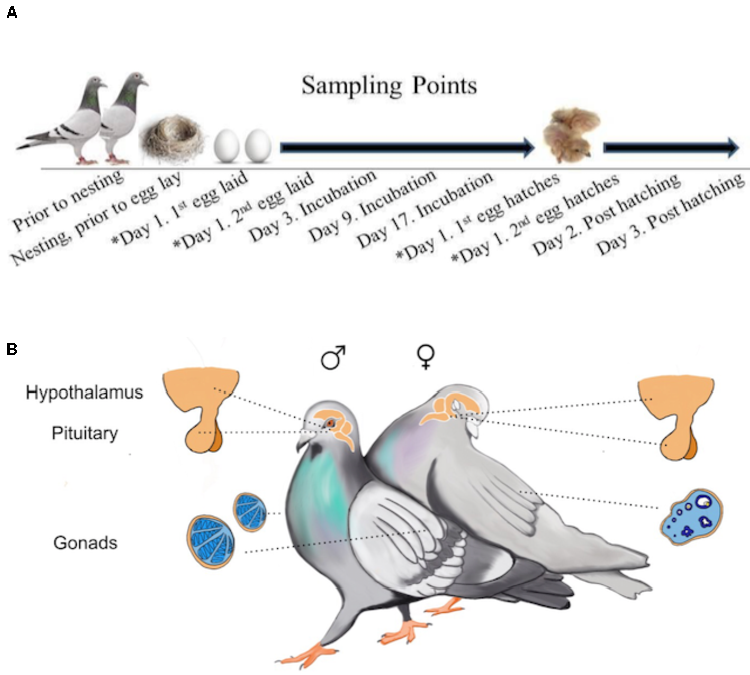
\includegraphics{characterization_manuscript_files/figure-latex/unnamed-chunk-2-1.pdf}
\caption{Experimental design.We sampled 9 timepoints, including 1
non-parental control, 1 nest-building, 1 egg lay, 3 incubation time
point, 1 hatch, and 2 nestling care stages. we collected truck blood,
the hypothalamus, the pituitary, and the gonads from all parents.}
\end{figure}

\begin{figure}
\centering
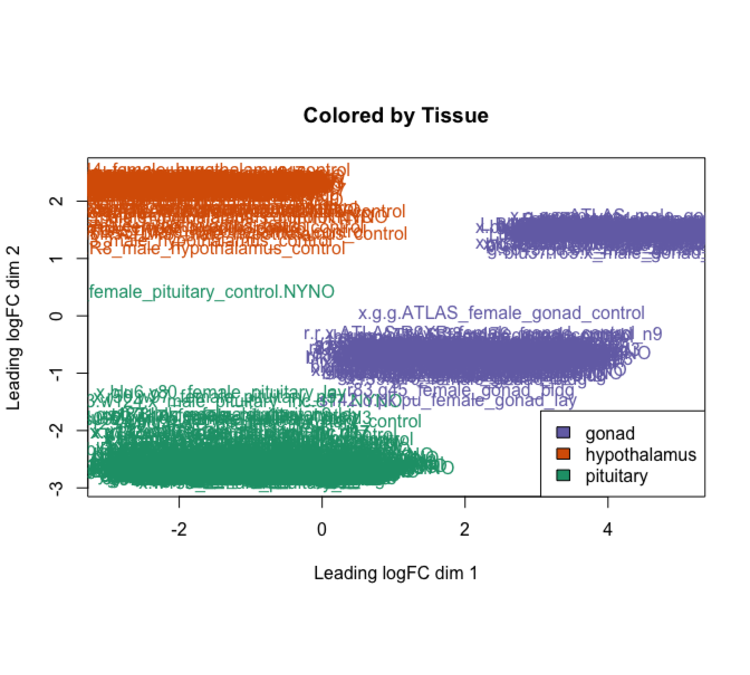
\includegraphics{characterization_manuscript_files/figure-latex/unnamed-chunk-3-1.pdf}
\caption{MDS plots of all samples. Needs improvement but shows that
tissue is source of main variation whereas sex really only affects the
gonads and treatment isn't noticable at this levels of analysis.}
\end{figure}

\begin{figure}
\centering
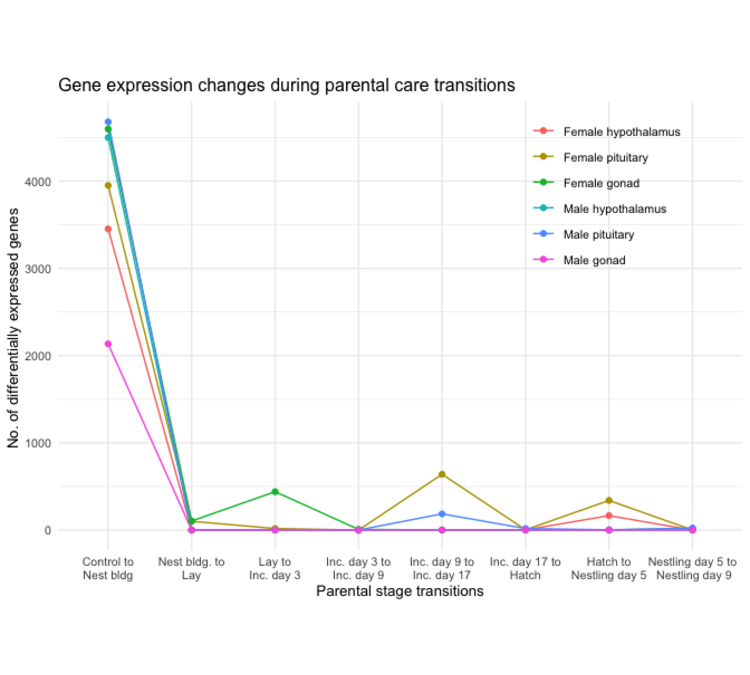
\includegraphics{characterization_manuscript_files/figure-latex/unnamed-chunk-4-1.pdf}
\caption{The magnitude of gene expression changes between each parental
transition. Using DESeq 2, we identified 4-5K genes are differentially
expressed beteen control birds and their nest buliding conspecifics in
all tissues except the male gonad. 500 - 1000 genes are differentially
expressed in the female pituitary from mid-late incubation as well as in
the female hypothalamus and pituitary from hatch to nestingly care day
5.}
\end{figure}

\begin{figure}
\centering
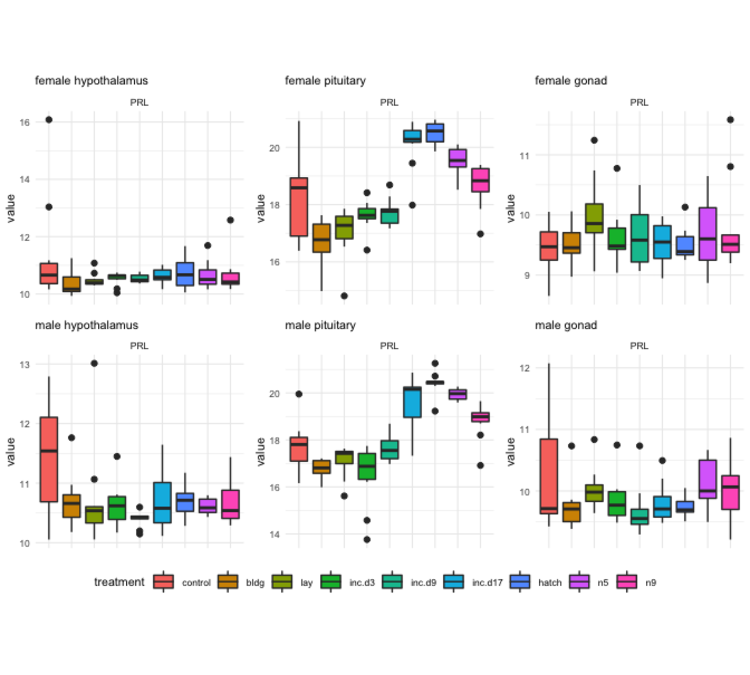
\includegraphics{characterization_manuscript_files/figure-latex/unnamed-chunk-5-1.pdf}
\caption{Linear discriminant analysis shows the strongest ability to
predict parental stage of pitutary samples.}
\end{figure}

\begin{figure}
\centering
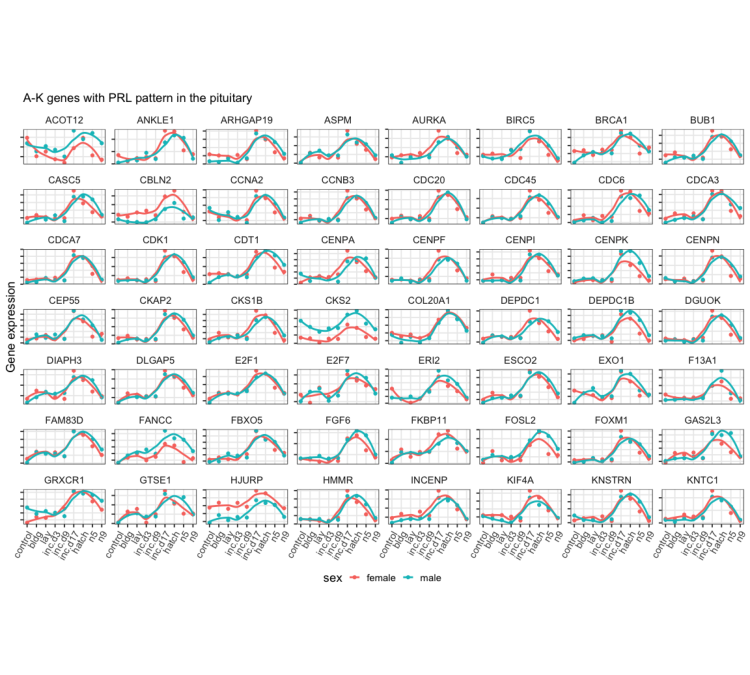
\includegraphics{characterization_manuscript_files/figure-latex/unnamed-chunk-6-1.pdf}
\caption{Prolactin expression in PIT (but not HYP or GON) follows same
pattern as in blood}
\end{figure}

\begin{figure}
\centering
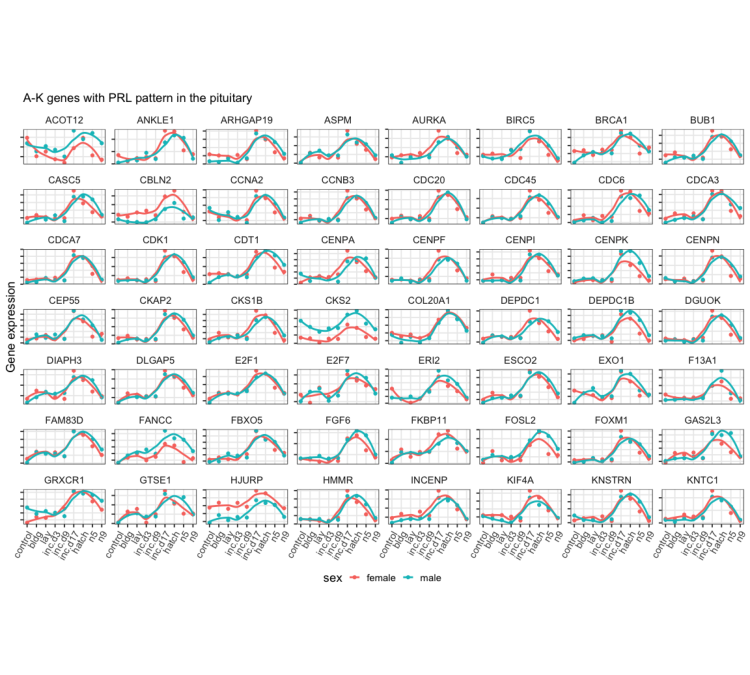
\includegraphics{characterization_manuscript_files/figure-latex/unnamed-chunk-7-1.pdf}
\caption{Hundreds of genes show similar pattern in expression as
circulating prolactin}
\end{figure}

\hypertarget{references}{%
\section*{References}\label{references}}
\addcontentsline{toc}{section}{References}

\hypertarget{refs}{}
\leavevmode\hypertarget{ref-Shapiro1063}{}%
1. Shapiro MD, Kronenberg Z, Li C, Domyan ET, Pan H, Campbell M, et al.
Genomic diversity and evolution of the head crest in the rock pigeon.
Science. American Association for the Advancement of Science; 2013;339:
1063--1067.
doi:\href{https://doi.org/10.1126/science.1230422}{10.1126/science.1230422}

\leavevmode\hypertarget{ref-Gillespie2012}{}%
2. Gillespie MJ, Stanley D, Chen H, Donald JA, Nicholas KR, Moore RJ, et
al. Functional Similarities between Pigeon `Milk' and Mammalian Milk:
Induction of Immune Gene Expression and Modification of the Microbiota.
Salmon H, editor. PLoS ONE. Public Library of Science; 2012;7: e48363.
doi:\href{https://doi.org/10.1371/journal.pone.0048363}{10.1371/journal.pone.0048363}

\nolinenumbers


\end{document}

